\ifdefined\ishandout
\documentclass[handout]{beamer}
\else
\documentclass{beamer}
\fi

\usepackage[frenchb]{babel}
\usepackage[T1]{fontenc}
\usepackage[latin1]{inputenc}
\usepackage{hyperref}
\usepackage{multirow}
\usepackage{listings}
\usepackage{fancyvrb}
\usepackage{tikz}
\usepackage{framed}
\usepackage{algorithm}
\usepackage{algorithmic}
\usepackage{xcolor}
\usepackage{color, colortbl}
\usepackage{handoutWithNotes}
\usetikzlibrary{shapes.geometric}
\usetikzlibrary{shapes.arrows, chains}
\usetikzlibrary{arrows,calc}
\usepackage{array}
\usetheme{Boadilla}

\ifdefined\ishandout
\pgfpagesuselayout{3 on 1 with notes}[a4paper,border shrink=5mm]
\usecolortheme{dove}
\else
\usecolortheme{dolphin}
\fi


\lstnewenvironment{codeC}
{ \lstset{language=C,
    otherkeywords={printf,scanf}}
}
{}

\ifdefined\ishandout
\definecolor{mygreen}{rgb}{0,0,0}
\definecolor{mymauve}{rgb}{0,0,0}
\definecolor{myblue}{rgb}{0,0,0}
\else
\definecolor{mygreen}{rgb}{0,0.6,0}
\definecolor{mymauve}{rgb}{0.58,0,0.82}
\definecolor{myblue}{rgb}{0,0,1}

\fi

\definecolor{mygray}{rgb}{0.5,0.5,0.5}


\lstset{language=C,
% breakatwhitespace=false,         % sets if automatic breaks should only happen at whitespace
%  breaklines=true,                 % sets automatic line breaking
%  captionpos=b,                
commentstyle=\itshape\color{mymauve},
keywordstyle=\bfseries\color{myblue},
%numbers=left,                    % where to put the line-numbers; possible values are (none, left, right)
%  numbersep=8pt,                   % how far the line-numbers are from the code
%  numberstyle=\tiny\color{mygray}, % the style that is used for the line-numbers
  rulecolor=\color{black},         % if not set, the frame-color may be changed on line-breaks within not-black text (e.g. comments (green here))
%  showspaces=false,                % show spaces everywhere adding particular underscores; it overrides 'showstringspaces'
  showstringspaces=false,          % underline spaces within strings only
%  showtabs=false,                  % show tabs within strings adding particular underscores
%  stepnumber=2,                    % the step between two line-numbers. If it's 1, each line will be numbered
  stringstyle=\color{mygreen},     % string literal style
%  tabsize=2 
}

\newcommand{\red}{\textcolor{red}}
%\newcommand \emph
%Default size : 12.8 cm * 9.6 cm

\ifdefined\ishandout
\newenvironment<>{codeblock}[1]{%begin
  \setbeamercolor{block title}{fg=black,bg=lightgray!80}%
  \begin{block}{#1}}
  % \begin{codeC}}
  %  {\end{codeC}
{  
\end{block}}

\newenvironment<>{termblock}[1]{
    \setbeamercolor{block title}{fg=black,bg=lightgray!90}%
    \begin{block}{#1}
}
%     \begin{Verbatim}}
{%\end{Verbatim}
\end{block}
}

\definecolor{bluegreen}{RGB}{0,0,0}
%\definecolor{bluegreen}{rgb}{0,0.6,0.8}
\else

\newenvironment<>{codeblock}[1]{%begin
  \setbeamercolor{block title}{fg=darkgray,bg=yellow}%
  \begin{block}{#1}}
  % \begin{codeC}}
  %  {\end{codeC}
{  
\end{block}}

\newenvironment<>{termblock}[1]{
    \setbeamercolor{block title}{fg=white,bg=lightgray}%
    \begin{block}{#1}}
%     \begin{Verbatim}}
{%\end{Verbatim}
\end{block}
}

\definecolor{bluegreen}{RGB}{0,149,182}
%\definecolor{bluegreen}{rgb}{0,0.6,0.8}
\fi

%\newcommand{\output}[1]{
\setbeamertemplate{navigation symbols}{}
\newcommand{\bvrb}{\Verb[commandchars=���,formatcom=\color{bluegreen}]}
\newcommand{\footvrb}{\footnotesize\Verb}


%%% Param�tres du cours (� r�gler)
%Num�ro du cours
\newcommand{\nb}{3}

\title[Cours n�\nb]{Cours n�\nb - Tableaux Statiques}
\author[]{julien.brajard@upmc.fr}
\institute[Polytech' UPMC]{Polytech' UPMC}
\date{03 Octobre 2016}
\begin{document}
%%%%%%%%%%%%%%%%%%%%% SLIDES DE TITRE
\begin{frame}
\titlepage
\centering{
\url{http://australe.upmc.fr} (onglet EPU-C5-IGE Info Gen)}
\end{frame}
%%%%%%%%%%%%%%%%%%%%%
\begin{frame}
\frametitle{Plan du cours n�\nb}
\tableofcontents[hideallsubsections]
\end{frame}

%%%%



%%%%%% SECTION 12
%% !TEX encoding = IsoLatin9

%%%%%%%%%%%%%%%%%%%%% SECTION 1
\section{La compilation}
\begin{frame}
  \begin{columns}
    \column{4.8cm}
    \tableofcontents[currentsection,hideothersubsections]
    \column{7cm}
    
  \end{columns}
  
\end{frame}

%%%%%%%%%%%%%%%%%%%%%%%%%%%%%%%%%%%%%%%%%%%
%                  FRAME 1                %
%%%%%%%%%%%%%%%%%%%%%%%%%%%%%%%%%%%%%%%%%%%

\begin{frame}[t,fragile]
\frametitle{Les 4 �tapes de la compilation}

%%%%%%%%%%%%%% ALL SLIDES %%%%%%%%%%%%%%%%%%
\vspace{-0.7cm}
\begin{figure}[t]
\centering
\begin{tikzpicture} [
  block/.style    = { rectangle, draw=blue, thick, 
                      fill=blue!20, text width=1.8cm, text centered,
                      rounded corners, minimum height=2em },
 ablock/.style    = { rectangle, draw=red, thick, 
                      fill=red!20, text width=1.8cm, text centered,
                      rounded corners, minimum height=2em },
 line/.style     = { draw, very thick, ->, shorten >=1pt },
 aline/.style     = { draw, color=red,very thick, ->, shorten >=1pt },
 label/.style    = {midway,anchor=north,yshift=-0.3cm, text width=2.4cm,text centered},
  node distance = 2.5cm,
]
\node <1-|handout:1-> (cfile) [block] {\Verb|Bonjour.c|};

\node <1,4-|handout:1,4-> (ifile) [block, right of = cfile] {\Verb|bonjour.i|};
\node <2-3|handout:2-3> (ifile) [ablock, right of = cfile] {\Verb|bonjour.i|};

\node <1-3,7-|handout:1-3,7->(sfile) [block, right of = ifile] {\Verb|bonjour.s|};
\node <4-6|handout:4-6> (sfile) [ablock, right of = ifile] {\Verb|bonjour.s|};

\node <1-6,8-|handout:1-6,8-> (ofile) [block, right of = sfile] {\Verb|bonjour.o|};
\node <7|handout:7> (ofile) [ablock, right of = sfile] {\Verb|bonjour.o|};

\node <1-7|handout:1-7> (efile) [block, right of = ofile] {\Verb|bonjour|};
\node <8|handout:8> (efile) [ablock, right of = ofile] {\Verb|bonjour|};

\path <1,4-|handout:1,4-> [line] (cfile) --  node[label]{preprocessing}(ifile) ;
\path <2-3|handout:2-3> [aline] (cfile) --  node[label]{preprocessing}(ifile) ;

\path <1-3,7-|handout:1-3,7-> [line] (ifile) -- node[label]{compilation}(sfile) ;
\path <4-6|handout:4-6> [aline] (ifile) -- node[label]{compilation}(sfile) ;

\path <1-6,8-|handout:1-6,8-> [line] (sfile) -- node[label]{assemblage}(ofile) ;
\path <7|handout:7> [aline] (sfile) -- node[label]{assemblage}(ofile) ;

\path <1-7|handout:1-7> [line] (ofile) -- node[label]{�dition des liens}(efile) ;
\path <8|handout:8> [aline] (ofile) -- node[label]{�dition des liens}(efile) ;

\end{tikzpicture}
\end{figure}
%%%%%%%%%%%%%% SLIDE 1 %%%%%%%%%%%%%%%%%%
\begin{overlayarea}{\textwidth}{5cm}


\begin{onlyenv}<1|handout:1>
\vspace{-0.9cm}
\begin{columns}[t]
\column{.33\textwidth}
\begin{codeblock}{\Verb|bonjour.c|\hfill\tikz[remember picture,baseline=-.5ex] \coordinate(b1);}
\vspace{-.3cm}
\tikz[remember picture,baseline=0ex] (tab) {X};
\lstset{escapeinside={��}}
\lstset{basicstyle=\scriptsize}
\begin{codeC}
#include <stdio.h>

int main () {
 // Affiche "bonjour"
 printf("bonjour\n");
}
\end{codeC}
\end{codeblock}

\column{.38\textwidth}
\begin{termblock}{\tikz[remember picture,baseline=-.5ex] \coordinate(b2);\Verb|Terminal|}
\vspace{-.3cm}
\lstset{escapeinside={��}}
\lstset{basicstyle=\scriptsize}
\begin{lstlisting}
�\textbf{>>}�gcc bonjour.c -o bonjour
\end{lstlisting}
\centering{\tikz[remember picture,baseline=-0.5ex] \coordinate(b2_south);}
\vspace{-.6cm}
\end{termblock}
\vspace{0.8cm}
\begin{block}{}
%\centering{\tikz[remember picture,baseline=-.5ex] \coordinate(b3);}\\
Fichier Ex�cutable \Verb|Bonjour|
\end{block}
\end{columns}

\begin{alertblock}{}
Par d�faut \Verb|gcc| effectue les 4 �tapes.
\end{alertblock}

\begin{tikzpicture}[remember picture,overlay]
\draw (b1) edge[->, very thick,shorten >=10pt, shorten <=10pt] (b2);
\draw ($(b2_south)+(0,0.6)$) edge[->, very thick,shorten >=10pt, shorten <=10pt] ++(0,-1.6);

\end{tikzpicture}

\end{onlyenv}

%%%%%%%%%%%%%% SLIDE 2 %%%%%%%%%%%%%%%%%
\begin{onlyenv}<2|handout:2>
\vspace{-0.9cm}

\begin{block}{Preprocessing}
Le pr�processeur effectue diff�rentes op�rations de substitution
et de supression dans le code :
\begin{itemize}
\item Supression des commentaires (\bvrb|//| et  \bvrb|/* */|)
qui sont utiles au programmeur, mais inutiles pour le processeur.\\
\item Inclusion des fichier \Verb|.h| dans le fichier \Verb|.c| 
(directive \bvrb|#include|). Ici, il permet de donner le prototype
de la fonction \bvrb|printf| (son format).\\
\item Traitemenet des directives de compilation qui commencent par
un caract�re \bvrb|#| (voir plus loin).\\
\end{itemize}

\end{block}
\end{onlyenv}

%%%%%%%%%%%%%% SLIDE 3 %%%%%%%%%%%%%%%%%%
\begin{onlyenv}<3|handout:3>
\vspace{-0.9cm}
\begin{columns}[t]
\column{.33\textwidth}
\begin{codeblock}{\Verb|bonjour.c|\hfill\tikz[remember picture,baseline=-.5ex] \coordinate(b1_2);}
\vspace{-.3cm}
\lstset{escapeinside={��}}
\lstset{basicstyle=\scriptsize}
\begin{codeC}
#include <stdio.h>

int main () {
 // Affiche "bonjour"
 printf("bonjour\n");
}
\end{codeC}
\end{codeblock}

\column{.6\textwidth}
\begin{termblock}{\tikz[remember picture,baseline=-.5ex] \coordinate(b2_2);\Verb|Terminal|}
\vspace{-.3cm}
\lstset{escapeinside={��}}
\lstset{basicstyle=\scriptsize}
\begin{lstlisting}
�\textbf{>>}�gcc -E Bonjour.c -o Bonjour.i
\end{lstlisting}
\centering{\tikz[remember picture,baseline=-0.5ex] \coordinate(b2_2_south);}
\vspace{-.6cm}
\end{termblock}
\vspace{0.2cm}
\begin{codeblock}{\Verb|bonjour.i|}
\vspace{-.3cm}
\lstset{escapeinside={��}}
\lstset{basicstyle=\scriptsize}
\begin{codeC}
(...) extern int printf 
 (__const char *__restrict__format, ...);
(...)
# 2 "bonjour.c" 2
int main () {
 printf("bonjour\n");
}
\end{codeC}
\end{codeblock}
\end{columns}

\begin{tikzpicture}[remember picture,overlay]
\draw (b1_2) edge[->, very thick,shorten >=3pt, shorten <=2pt] (b2_2);
\draw ($(b2_2_south)+(0,0.6)$) edge[->, very thick , shorten <=10pt] ++(0,-0.7);

\end{tikzpicture}

\end{onlyenv}


%%%%%%%%%%%%%% SLIDE 4 %%%%%%%%%%%%%%%%%%
\begin{onlyenv}<4|handout:4>
\begin{block}{La compilation}
La compilation (au sens strict) tranforme le langage C en assembleur.
\end{block}
\end{onlyenv}



%%%%%%%%%%%%%% SLIDE 5 %%%%%%%%%%%%%%%%%%
\begin{onlyenv}<5|handout:5>

\vspace{-0.9cm}
\begin{columns}[t]
\column{.33\textwidth}
\begin{codeblock}{\Verb|bonjour.c|\hfill\tikz[remember picture,baseline=-.5ex] \coordinate(b1_2);}
\vspace{-.3cm}
\lstset{escapeinside={��}}
\lstset{basicstyle=\scriptsize}
\begin{codeC}
#include <stdio.h>

int main () {
 // Affiche "bonjour"
 printf("bonjour\n");
}
\end{codeC}
\end{codeblock}

\column{.6\textwidth}
\begin{termblock}{\tikz[remember picture,baseline=-.5ex] \coordinate(b2_2);\Verb|Terminal|}
\vspace{-.3cm}
\lstset{escapeinside={��}}
\lstset{basicstyle=\scriptsize}
\begin{lstlisting}
�\textbf{>>}�gcc -S Bonjour.c -o bonjour.s
\end{lstlisting}
\centering{\tikz[remember picture,baseline=-0.5ex] \coordinate(b2_2_south);}
\vspace{-.6cm}
\end{termblock}

\vspace{0.2cm}

\begin{codeblock}{\Verb|bonjour.s|}
\vspace{-.3cm}
\lstset{escapeinside={��}}
\lstset{basicstyle=\scriptsize}
\begin{codeC}
	.file	"bonjour.c"
	.section	.rodata
.LC0:
	.string	"bonjour"
(...)
	movl	$.LC0, %edi
	call	puts
(...)
	.section	.note.GNU-stack,"",@progbits
\end{codeC}
%$
\end{codeblock}
\end{columns}

\begin{tikzpicture}[remember picture,overlay]
\draw (b1_2) edge[->, very thick,shorten >=3pt, shorten <=2pt] (b2_2);
\draw ($(b2_2_south)+(0,0.6)$) edge[->, very thick , shorten <=10pt] ++(0,-0.7);

\end{tikzpicture}

\end{onlyenv}


%%%%%%%%%%%%%% SLIDE 6 %%%%%%%%%%%%%%%%%%
\begin{onlyenv}<6|handout:6>
\vspace{-3.9cm}
\begin{codeblock}{\Verb|bonjour.s| complet !}
\vspace{-.3cm}
\lstset{escapeinside={��}}
\lstset{basicstyle=\scriptsize}
\begin{codeC}
	.file	"bonjour.c"
	.section	.rodata
.LC0:
	.string	"bonjour"
	.text
	.globl	main
	.type	main, @function
main:
.LFB0:
	.cfi_startproc
	pushq	%rbp
	.cfi_def_cfa_offset 16
	.cfi_offset 6, -16
	movq	%rsp, %rbp
	.cfi_def_cfa_register 6
	movl	$.LC0, %edi
	call	puts
	popq	%rbp
	.cfi_def_cfa 7, 8
	ret
	.cfi_endproc
.LFE0:
	.size	main, .-main
	.ident	"GCC: (Ubuntu/Linaro 4.6.3-1ubuntu5) 4.6.3"
	.section	.note.GNU-stack,"",@progbits
\end{codeC}
%$
\vspace{-0.3cm}
\end{codeblock}

\end{onlyenv}


%%%%%%%%%%%%%% SLIDE 7 %%%%%%%%%%%%%%%%%%
\begin{onlyenv}<7|handout:7>

\vspace{-0.9cm}
\begin{block}{}
Le code assembleur (encore lisible) est transform�
en code machine binaire.
\end{block}
\begin{columns}[t]
\column{.33\textwidth}
\begin{codeblock}{\Verb|bonjour.s|\hfill\tikz[remember picture,baseline=-.5ex] \coordinate(b1_2);}
\vspace{-.3cm}
\lstset{escapeinside={��}}
\lstset{basicstyle=\scriptsize}
\begin{codeC}
	.file	"bonjour.c"
	.section	.rodata
.LC0:
	.string	"bonjour"
(...)
	movl	$.LC0, %edi
	call	puts
(...)
	.section	
 .note.GNU-stack,"",
 @progbits
\end{codeC}
%$
\vspace{-0.3cm}
\end{codeblock}

\column{.6\textwidth}
\begin{termblock}{\tikz[remember picture,baseline=-.5ex] \coordinate(b2_2);\Verb|Terminal|}
\vspace{-.3cm}
\lstset{escapeinside={��}}
\lstset{basicstyle=\scriptsize}
\begin{lstlisting}
�\textbf{>>}�gcc -c bonjour.s
�\textbf{>>}�od -x bonjour.o
\end{lstlisting}
\centering{\tikz[remember picture,baseline=-0.5ex] \coordinate(b2_2_south);}
\vspace{-.6cm}
\end{termblock}

\vspace{0.2cm}

\begin{termblock}{\Verb|bonjour.o|}
\vspace{-.3cm}
\lstset{escapeinside={��}}
\lstset{basicstyle=\tiny}
\begin{lstlisting}
0000000 457f 464c 0102 0001 0000 0000 0000 0000
0000020 0001 003e 0001 0000 0000 0000 0000 0000
0000040 0000 0000 0000 0000 0128 0000 0000 0000
...
\end{lstlisting}
\end{termblock}
\end{columns}

\begin{tikzpicture}[remember picture,overlay]
\draw (b1_2) edge[->, very thick,shorten >=3pt, shorten <=2pt] (b2_2);
\draw ($(b2_2_south)+(0,0.6)$) edge[->, very thick , shorten <=10pt] ++(0,-0.7);

\end{tikzpicture}

\end{onlyenv}

%%%%%%%%%%%%%% SLIDE 8 %%%%%%%%%%%%%%%%%%
\begin{onlyenv}<8|handout:8>

\vspace{-0.9cm}
\begin{block}{}
Le fichier \Verb|bonjour.o| est incomplet, il manque le code
correspondant aux fonctions des biblioth�ques (ici : la fonction
\bvrb|printf| de la biblioth�que \Verb|stdio.h|).
\end{block}
\begin{columns}[t]
\column{.33\textwidth}
\begin{termblock}{\Verb|bonjour.o|\hfill\tikz[remember picture,baseline=-.5ex] \coordinate(b1_2);}
\Verb|(code binaire)|
\end{termblock}


\column{.6\textwidth}
\begin{termblock}{\tikz[remember picture,baseline=-.5ex] \coordinate(b2_2);\Verb|Terminal|}
\vspace{-.3cm}
\lstset{escapeinside={��}}
%\lstset{basicstyle=\scriptsize}
\begin{lstlisting}
�\textbf{>>}�gcc bonjour.o -o bonjour
\end{lstlisting}
\centering{\tikz[remember picture,baseline=-0.5ex] \coordinate(b2_2_south);}
\vspace{-.6cm}
\end{termblock}

\vspace{0.2cm}

\begin{termblock}{\Verb|bonjour|}
Fichier ex�cutable
\end{termblock}

\end{columns}

\begin{tikzpicture}[remember picture,overlay]
\draw (b1_2) edge[->, very thick,shorten >=3pt, shorten <=2pt] (b2_2);
\draw ($(b2_2_south)+(0,0.6)$) edge[->, very thick , shorten <=10pt] ++(0,-0.7);

\end{tikzpicture}


\end{onlyenv}
\end{overlayarea}

\end{frame}

%%%%%%%%%%%%%%%%%%%%%%%%%%%%%%%%%%%%%%%%%%%
%                  FRAME 2                %
%%%%%%%%%%%%%%%%%%%%%%%%%%%%%%%%%%%%%%%%%%%
\begin{frame}[fragile]
\frametitle{La directive \bvrb|\#define|}
%\frametitle{L'instruction \bvrb|if...else|}


\begin{itemize}
\item D�claration de constantes (ou d'une expression fixe quelconque) :\\
\bvrb|#define �textit�identificateur reste_de_la_ligne�|\\
\item Lorsque le pr�processeur lit une ligne de ce type, il remplace
toutes les occurences suivantes de \bvrb|�textit�identificateur�| dans le fichier texte
par \bvrb|�textit�reste_de_la_ligne�|\\
\item Par convention, on �crit l'identificateur en MAJUSCULE.
\end{itemize}
\begin{columns}
\column{0.3\textwidth}
\begin{codeblock}{\Verb|exemple.c|\hfill\tikz[remember picture,baseline=-.5ex] \coordinate(lc);}
%\vspace{-.3cm}
\lstset{escapeinside={��}}
\lstset{basicstyle=\scriptsize}
\begin{codeC}
#define PI 3.14159

int main()
{
  int x;
  x = PI*2 ;
}
\end{codeC}
\end{codeblock}
\column{0.3\textwidth}

\begin{termblock}{\tikz[remember picture,baseline=-.5ex] \coordinate(li);\Verb|Terminal|}
\vspace{-.3cm}
\lstset{escapeinside={��}}
\lstset{basicstyle=\scriptsize}
\begin{lstlisting}
�\textbf{>>}� gcc -E exemple.c 
  > exemple.i
\end{lstlisting}
\end{termblock}
\column{0.3\textwidth}
\begin{codeblock}{\tikz[remember picture,baseline=-.5ex] \coordinate(li);\Verb|exemple.i|}
%\vspace{-.3cm}
\lstset{escapeinside={��}}
\lstset{basicstyle=\scriptsize}
\begin{codeC}
# 2 "exemple.c" 2

int main()
{
  int x;
  x = 3.14159*2 ;
}
\end{codeC}
\end{codeblock}
\end{columns}

\begin{tikzpicture}[remember picture,overlay]
\draw (lc) edge[->, very thick,shorten >=6pt, shorten <=6pt] (li);


\end{tikzpicture}

\end{frame}

\begin{frame}[fragile]
\frametitle{Conseils sur le \bvrb|\#define|}
\begin{itemize}
\item Il est fortement recommand� de placer les
\bvrb|#define| au d�but de votre programme au m�me endroit
que les \bvrb|#include|.\\
\item Limitez l'utilisation des \bvrb|#define| � des options de
compilation ou � des constantes valables et utilis�es dans tout le
programme.\\
\end{itemize}
\begin{columns}
\column{0.4\textwidth}
\begin{flushright}
Placer ici les \bvrb|#define| de vos programmes.
\tikz[remember picture,baseline=-.5ex]\coordinate(left);
\end{flushright}

\column{0.4\textwidth}
\begin{codeblock}{}
%\vspace{-.3cm}
\lstset{escapeinside={��}}
\lstset{basicstyle=\scriptsize}
\begin{codeC}
#include <stdio.h>
�\tikz[remember picture,baseline=-.5ex]\coordinate(d1);�#define PI 3.14159
�\tikz[remember picture,baseline=-.5ex]\coordinate(d2);�#define NMAX 500
�\tikz[remember picture,baseline=-.5ex]\coordinate(d3);�#define DEBUG_MODE

int main()
{
...
}
\end{codeC}
\end{codeblock}
\end{columns}


\begin{tikzpicture}[remember picture,overlay]
\draw (left) edge[->, gray, thick,shorten >=2pt, shorten <=2pt] (d1);
\draw (left) edge[->, gray, thick,shorten >=2pt, shorten <=2pt] (d2);
\draw (left) edge[->, gray, thick,shorten >=2pt, shorten <=2pt] (d3);
\end{tikzpicture}

\end{frame}

\begin{frame}[fragile]
\frametitle{Les directives pour le pr�processeur}
\begin{itemize}
\item \bvrb|#define �textit�identificateur reste_de_la_ligne�|\\
Remplace \bvrb|�textit�identificateur�| par  \bvrb|�textit�reste_de_la_ligne�|
jusqu'� la fin du programme ou jusqu'� une instruction \bvrb|#undef|.\\
\vspace{0.5cm}
\item \bvrb|#undef �textit�identificateur�|\\
Marque la fin du remplacement syst�matique initi� par \bvrb|#define|\\
\vspace{0.5cm}

\item \bvrb|#ifdef �textit�identificateur� ... #endif|\\
Inlus la partie de programme situ�e entre \bvrb|#ifdef| et \bvrb|#endif| si
l'identificateur a �t� d�clar� avant dans un \bvrb|#define|. Sinon, la partie de
programme concern�e est supprim�e avant compilation.\\
\end{itemize}

\end{frame}

\begin{frame}[fragile]
\frametitle{Exemple}

\begin{columns}

\column{.48\textwidth}
\begin{codeblock}{\centering{\Verb|exemple.c|\tikz[remember picture,baseline=-.5ex] \coordinate(lc);}}
\lstset{escapeinside={��}}
\lstset{basicstyle=\scriptsize}
\begin{codeC}
#define PI 3.14159

int main()
{
  int x;
  x = PI*2;
#ifdef PI
  printf("Constante PI d�finie");
#endif
  printf("x=%f",x);
#undef PI
#ifdef PI
  printf("Ce printf sera supprim�
par le pr�processeur");
#endif
}
\end{codeC}
\end{codeblock}

\column{.48\textwidth}
\begin{codeblock}{\centering{\tikz[remember picture,baseline=-.5ex] \coordinate(li);\Verb|exemple.i|}}
\lstset{escapeinside={��}}
\lstset{basicstyle=\scriptsize}
\begin{codeC}
#2 exemple.c 2

int main()
{
  int x;
  x = PI*2;

  printf("Constante PI d�finie");

  printf("x=%f",x);





}
\end{codeC}
\end{codeblock}

\end{columns}

\begin{tikzpicture}[remember picture,overlay]
\draw (lc) edge[->, very thick,shorten >=6pt, shorten <=6pt] (li);
\end{tikzpicture}


\end{frame}
%% !TEX encoding = IsoLatin9

%%%%%%%%%%%%%%%%%%%%% SECTION 1
\section{Entr�es/Sorties}
\begin{frame}
  \begin{columns}
    \column{4.8cm}
    \tableofcontents[currentsection,hideothersubsections]
    \column{7cm}
     \centering{
      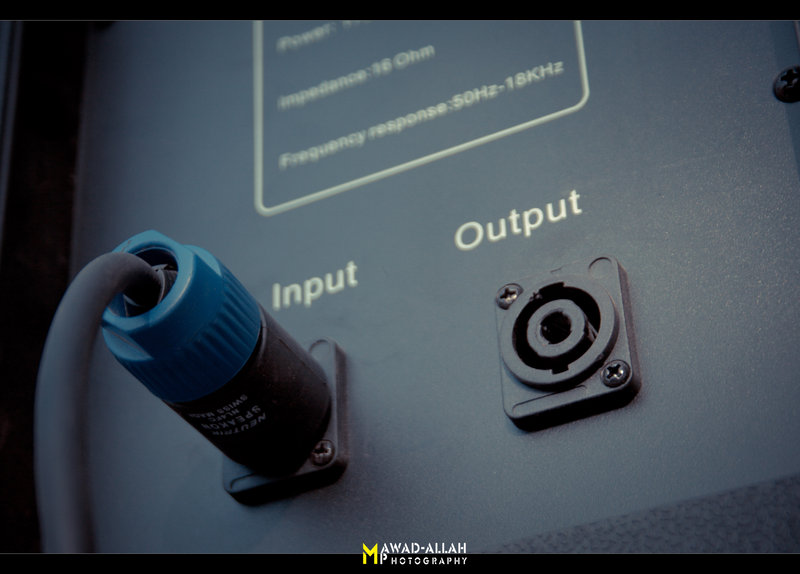
\includegraphics[width=5cm]{fig/inout.jpg}
}
  \end{columns}
  
\end{frame}

\begin{frame}[fragile]
\frametitle{Les entr�es/sorties}
\begin{itemize}
\item Affichage de caract�res � l'�cran : \\
\bvrb|printf(�textit�chaine_de_caracteres�,�textit�variables�);|\\
\vspace{0.5cm}
\item Lecture de caract�res au clavier : \\
\bvrb|scanf(�textit�format�,�textit�adresses�);|\\
\vspace{0.5cm}
\item Pour utiliser ces fonctions, il est n�cessaire d'inclure au programme
la biblioth�que \Verb|stdio.h| g�rant les entr�es sorties :
\begin{codeblock}{}
\lstset{escapeinside={��}}
%\lstset{basicstyle=\scriptsize}
\begin{codeC}
#include <stdio.h>
\end{codeC}
\end{codeblock}

\end{itemize}
\end{frame}

\begin{frame}[fragile]
\frametitle{Comment fonctionne le \bvrb|scanf| ?}
\begin{figure}
\centering
\begin{tikzpicture} [
  auto,
  line/.style     = { draw, thick, color=red,->, shorten >=2pt },
  node distance = 4cm
]
\node[inner sep=0pt] (clavier)
{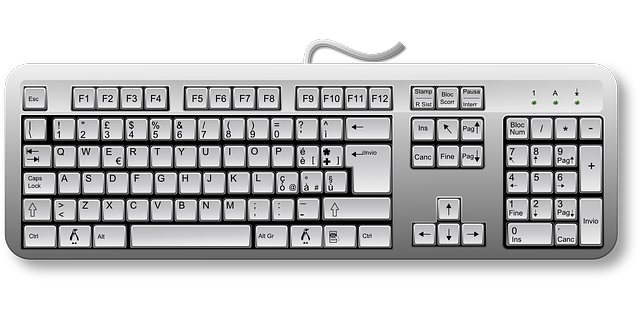
\includegraphics[width=3cm]{./fig/clavier.png}};
\node[inner sep=0pt,right of=clavier] (fils) 
{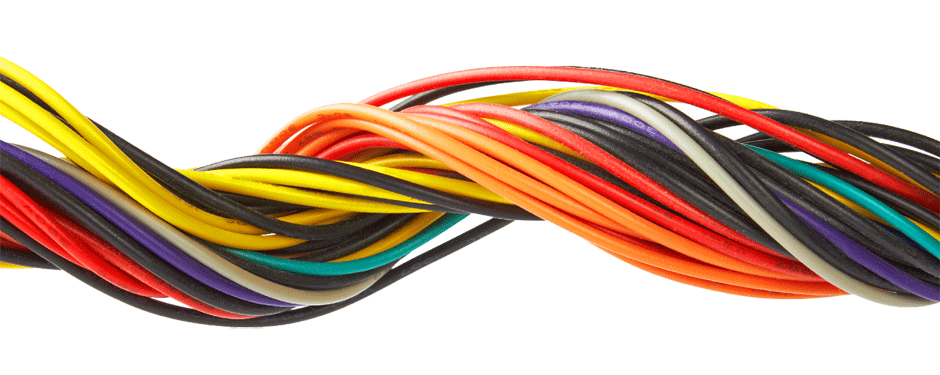
\includegraphics[width=3cm]{./fig/cables.png}};
\node[inner sep=0pt,right of=fils] (proc) 
{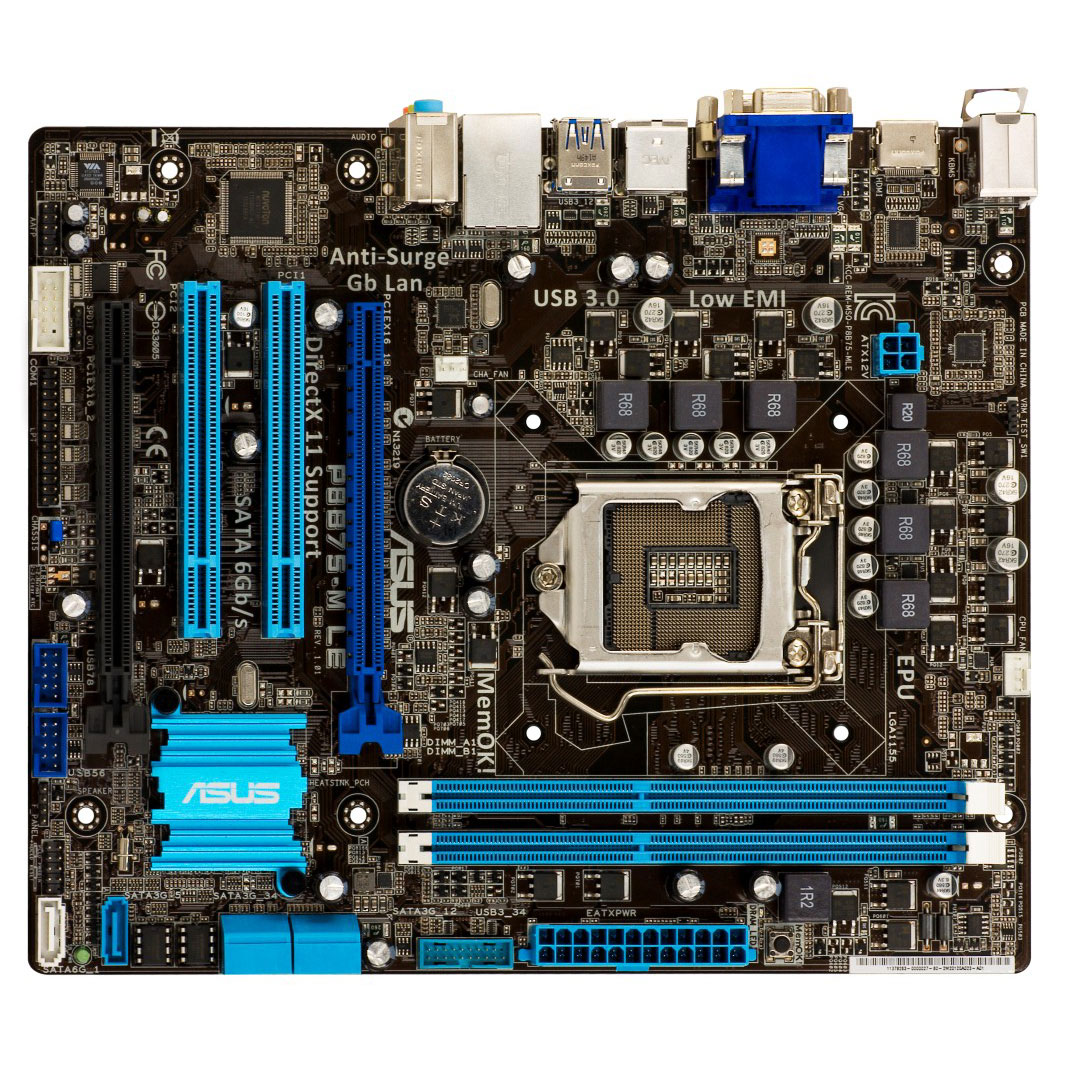
\includegraphics[width=3cm]{./fig/carte_mere.jpg}};
\node [below of = clavier,yshift = +2cm] (input) {{\Large 5}};
\node [below of = proc, yshift  = +2cm] (mem)
{
  \begin{tabular}{p{0.9em}|p{0.9em}|p{0.9em}|p{0.9em}|p{0.9em}}
    \hline
    ... & & 5 & & ... \\
    \hline
    \multicolumn{2}{p{1.8em}}{} &\multicolumn{1}{p{0.9em}}{\texttt{\&n}} & \multicolumn{2}{p{1.8em}}{}  \\
  \end{tabular}
};
\path [line] (input) -- (mem);
\end{tikzpicture}
\end{figure}

\begin{columns}
\column{0.45\textwidth}
\begin{codeblock}{}
\lstset{escapeinside={��}}
%\lstset{basicstyle=\scriptsize}
\begin{codeC}
scanf("%d",&n);
\end{codeC}
\end{codeblock}
\column{0.45\textwidth}
La valeur 5 est affect�e � la variable \Verb|n|.

La case m�moire adress�e par \Verb|&n| contient la 
valeur 5
\end{columns}


\end{frame}


\begin{frame}[fragile]
\frametitle{Comment fonctionne le \bvrb|printf| ?}
\begin{figure}
\centering
\begin{tikzpicture} [
  auto,
  line/.style     = { draw, color=red, thick, ->, shorten >=2pt },
  node distance = 4cm
]
\node[inner sep=0pt] (proc) 
{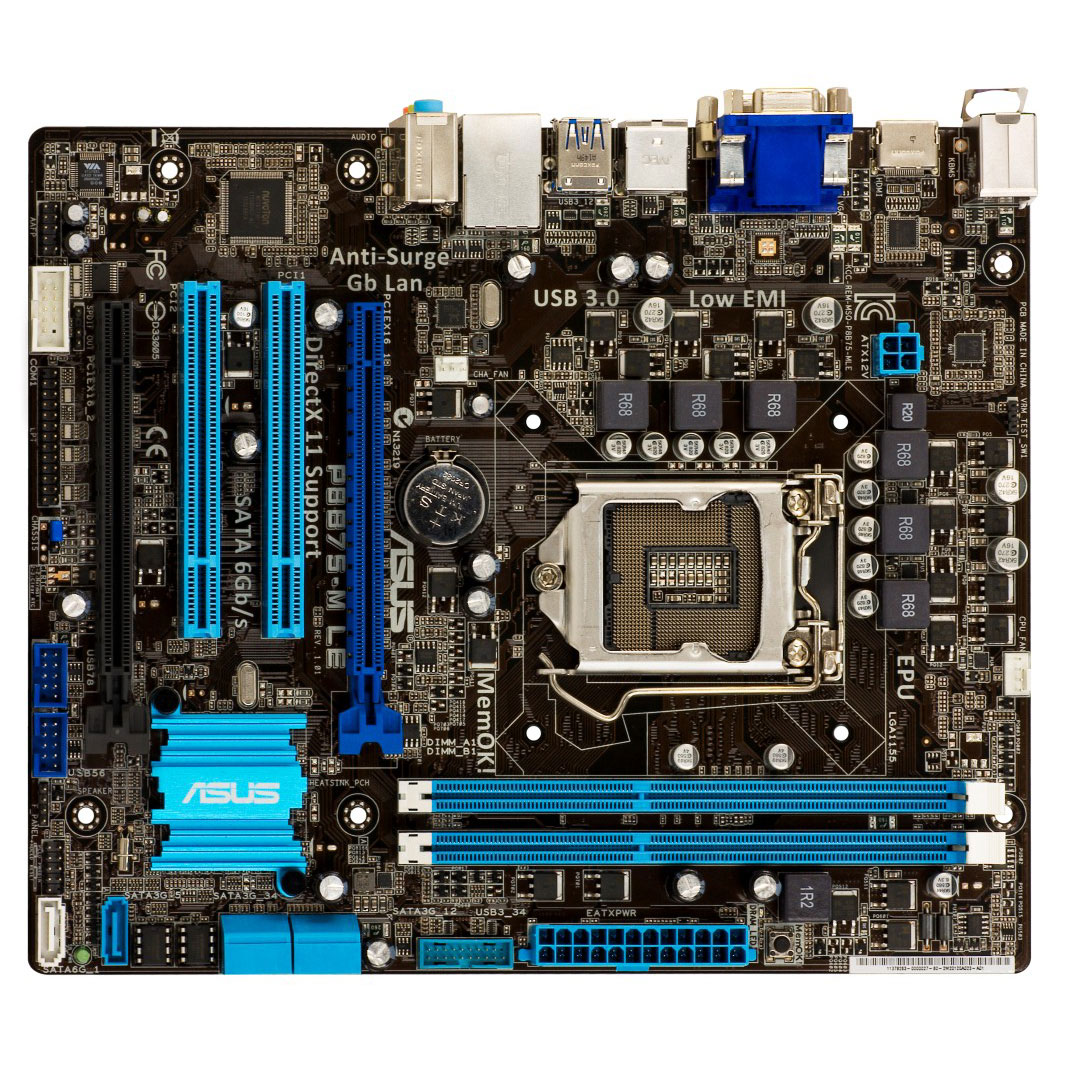
\includegraphics[width=3cm]{./fig/carte_mere.jpg}};
\node[inner sep=0pt,right of=proc] (fils) 
{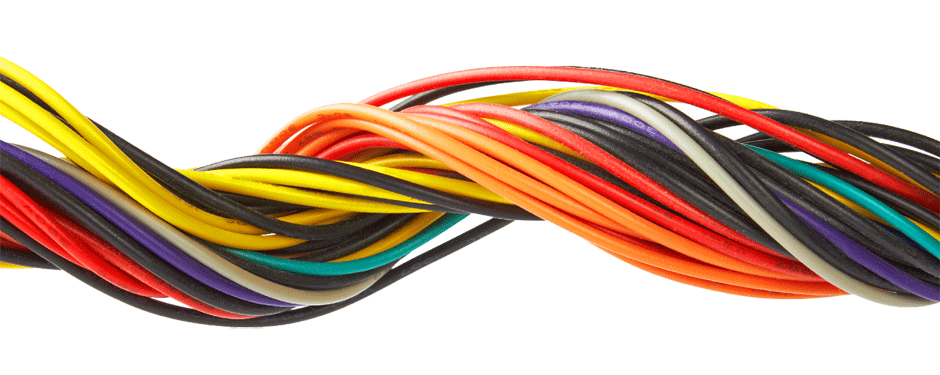
\includegraphics[width=3cm]{./fig/cables.png}};
\node[inner sep=0pt, right of=fils] (ecran)
{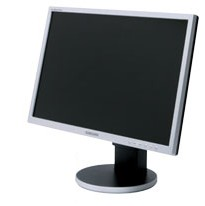
\includegraphics[width=3cm]{./fig/ecran.jpg}};

\node [below of = ecran,yshift = +2cm] (output) {{\Large 5}};
\node [below of = proc, yshift  = +2cm] (mem)
{
  \begin{tabular}{p{0.9em}|p{0.9em}|p{0.9em}|p{0.9em}|p{0.9em}}
    \hline
    ... & & 5 & & ... \\
    \hline
    \multicolumn{2}{p{1.8em}}{} &\multicolumn{1}{p{0.9em}}{\texttt{\&n}} & \multicolumn{2}{p{1.8em}}{}  \\
  \end{tabular}
};
\path [line] (mem) -- (output);
\end{tikzpicture}
\end{figure}

\begin{columns}
\column{0.45\textwidth}
\begin{codeblock}{}
\lstset{escapeinside={��}}
%\lstset{basicstyle=\scriptsize}
\begin{codeC}
printf("%d",n);
\end{codeC}
\end{codeblock}
\column{0.45\textwidth}
Affiche la valeur de la variable \Verb|n|.

La case m�moire adress�e par \Verb|&n| est affich�.
\end{columns}


\end{frame}

\begin{frame}[fragile]
\frametitle{Les codes formats}
\begin{table}
\begin{tabular}{|l|l|}
\hline
\bvrb|%c| & Caract�re \\
\hline
\bvrb|%d| & Entier sign� \\
\hline
\bvrb|%u| & Entier non sign� \\
\hline
\bvrb|%x| ou \bvrb|%X| & Entier en hexad�cimal \\
\hline
\bvrb|%o| & Entier en octal\\
\hline
\bvrb|%ld| & Entier long sign� \\
\hline
\bvrb|%lu| & Entier long non sign� \\
\hline
\bvrb|%lx| ou \bvrb|%lX| & Entier long en hexad�cimal \\
\hline
\bvrb|%f| & R�el simple pr�cision avec virgule flottante \\
\hline
\bvrb|%e| ou \bvrb|%E| & R�el simple pr�cision avec exposant e ou E \\
\hline
\bvrb|%lf| & R�el double avec virgule flottante \\
\hline
\bvrb|%le| ou \bvrb|%lE| & R�el double avec exposant e ou E \\
\hline
\bvrb|%Lf| & R�el long double avec virgule flottante \\
\hline
\bvrb|%Le| ou \bvrb|%LE| & R�el long double avec exposant e ou E \\
\hline
\bvrb|%s| & Cha�ne de caract�res \\
\hline
\bvrb|%p| & Pointeur \\
\hline
\end{tabular}
\end{table}

\end{frame}

\begin{frame}[fragile]
\frametitle{Compl�ments sur les formats}

\begin{itemize}
\item Autres formats d'affichage :\\
\begin{description}
\item[]\bvrb|\n| : Passage � la ligne.\\
\item[]\bvrb|\t| : Tabulation.\\
\item[]\bvrb|\0| : Fin de cha�ne.\\
\item[]\bvrb|\%| : Signe pourcentage.\\
\end{description}
\item On peut pr�c�der les codes des r�els de deux entiers : \bvrb|%n.p|
\begin{description}
\item[]\bvrb|n| : largeur minimale \\
\item[]\bvrb|p| : pr�cisions \\
\end{description}
\item On peut pr�c�der les codes des entiers d'un entier :
\begin{description}
\item[]\bvrb|%n| : largeur minimale de n.\\
\item[]\bvrb|%0n| : largeur minimal de n avec les blancs combl�s par des z�ros.\\
\end{description}

\end{itemize}

\end{frame}

\begin{frame}[fragile]
\frametitle{Exemples}

\begin{codeblock}{}
\lstset{escapeinside={��}}
%\lstset{basicstyle=\scriptsize}
\begin{codeC}
 int n=34 ;
 float x = 3.1,y=1.525;
 printf("_%d_%3d_%1d_%03d_\n",n,n,n,n);
 printf("_%f_%3.2f_\n",x,x);
 printf("_%f_%5.2f_%2.2f_\n",y,y,y);
\end{codeC}
\end{codeblock}
\begin{termblock}{Test d'ex�cution}
\lstset{escapeinside={��}}
\begin{Verbatim}
_34_ 34_34_034_
_3.100000_3.10_
_1.525000_ 1.52_1.52_
\end{Verbatim}
\end{termblock}


\end{frame}

\begin{frame}[fragile]
\frametitle{\bvrb|scanf| : comment �a se passe ?}
\begin{codeblock}{}
\vspace{-0.2cm}
\lstset{escapeinside={��}}
%\lstset{basicstyle=\scriptsize}
\begin{codeC}
int a; float x ;
scanf("%d %f",&a,&x);
\end{codeC}
\vspace{-0.2cm}
\end{codeblock}
\begin{enumerate}[<+->]
\item Si le tampon est vide, le programme s'interrompt pour laisser
l'utilisateur taper au clavier.\\
\item D�s que la touche \Verb|Entr�e| est frapp�e, la s�quence des �lements
entr�s est stock�e dans une zone m�moire appel�e \red{tampon}.\\
\item La directive \bvrb|scanf| consomme la m�moire tampon en fonction
du format indiqu� et stocke les �l�ments convertis dans les variables :\\
\begin{itemize}
\item Si le tampon est vide avant que le format du \bvrb|scanf| ne soit
enti�rement converti, on retourne � l'�tape 1.\\
\item Si le format dans le \bvrb|scanf| ne correspond pas au prochain caract�re de la s�quence
entr�e au clavier, \red{la conversion s'interrompt et le programme continue}.\\
\item Si la conversion est enti�rement termin�e, le programme continue
mais \red{il peut rester encore des �l�ments dans le tampon}.\\
\end{itemize}
\end{enumerate}

\end{frame}

\begin{frame}[t,fragile]
\frametitle{Illustration}
\begin{columns}[t]
\column{0.4\textwidth}
\begin{codeblock}{}
\vspace{-0.2cm}
\lstset{escapeinside={��}}
%\lstset{basicstyle=\scriptsize}
\begin{codeC}
int a; float x ;
scanf("%d %f",&a,&x);�\tikz[remember picture,baseline=-.5ex]\coordinate(code);�
\end{codeC}
\vspace{-0.2cm}
\end{codeblock}
\vspace{0.5cm}
\begin{visibleenv}<3->
\begin{termblock}{au clavier : \tikz[remember picture,baseline=-.5ex]\coordinate(clav);   }
\lstset{escapeinside={��}}
\begin{lstlisting}
3 2.5 (Entr�e)�\tikz[remember picture,baseline=-.5ex]\coordinate(term);�
\end{lstlisting}
\end{termblock}
\vspace{0.4cm}
\end{visibleenv}

\begin{visibleenv}<6->

L'espace est ignor� \tikz[remember picture,baseline=-.5ex]\coordinate(space);\\
\red{sauf} si le format \bvrb|%c|
(caract�re) est sp�cifi�.
\end{visibleenv}

\column{0.55\textwidth}
\vspace{-0.5cm}
\begin{figure}
  % \centering
  \begin{tikzpicture}[
    auto,
    remember picture,
    node distance = 2cm,
    fond/.style = {rectangle,draw=blue!80, rectangle, minimum width=5.5cm, minimum height = 1.5cm, fill=blue!20},
    head/.style={regular polygon, xshift=-2.27cm,yshift=0.13cm,fill=black,rotate around = {60:(0,0)},regular polygon sides = 3, inner sep=0.05cm},
    ]
    \node <2->(boite1) [fond]{};
    \node <4->(boite2) [fond,below of = boite1]{};
    \node <5->(boite3) [fond,below of = boite2]{};
    \node <7->(boite4) [fond,below of = boite3]{};
    
    \node <2->(tampon1)
    {
      \begin{tabular}{|p{0.35cm}|p{0.35cm}|p{0.35cm}|p{0.35cm}|p{0.1cm}|p{0.35cm}|p{0.35cm}|}
        \multicolumn{4}{c}{tampon}& \multicolumn{1}{c}{} & \multicolumn{1}{c}{\texttt{\&a}} & \multicolumn{1}{c}{\texttt{\&x}} \\
        \cline{1-4}\cline{6-7}
        & & & & & & \\
        \cline{1-4}\cline{6-7}
      \end{tabular}
    };
    \node <2-> (tik1) [head] {};
    
    \node <4-> (tampon2) [below of = boite1]
    {
      \begin{tabular}{|p{0.35cm}|p{0.35cm}|p{0.35cm}|p{0.35cm}|p{0.1cm}|p{0.35cm}|p{0.35cm}|}
        \multicolumn{4}{c}{tampon}& \multicolumn{1}{c}{} & \multicolumn{1}{c}{\texttt{\&a}} & \multicolumn{1}{c}{\texttt{\&x}} \\
        \cline{1-4}\cline{6-7}
        \footvrb|3| & & \footvrb|2.5| & \footvrb|\n| & & & \\
        \cline{1-4}\cline{6-7}
      \end{tabular}
    };

\node <4->(tik2) [below of =boite1, head] {};
        \node  <5-> (tampon3) [below of = boite2]
    {
      \begin{tabular}{|p{0.35cm}|p{0.35cm}|p{0.35cm}|p{0.35cm}|p{0.1cm}|p{0.35cm}|p{0.35cm}|}
        \multicolumn{4}{c}{tampon}& \multicolumn{1}{c}{} & \multicolumn{1}{c}{\texttt{\&a}} & \multicolumn{1}{c}{\texttt{\&x}} \\
        \cline{1-4}\cline{6-7}
        & \footvrb|2.5| & \footvrb|\n| & & & 3 & \\
        \cline{1-4}\cline{6-7}
      \end{tabular}
    };
    \node <5->(tik3) [below of =boite2, head] {};
    \node <7->(tampon4) [below of = boite3]
    {
      \begin{tabular}{|p{0.35cm}|p{0.35cm}|p{0.35cm}|p{0.35cm}|p{0.1cm}|p{0.35cm}|p{0.35cm}|}
        \multicolumn{4}{c}{tampon}& \multicolumn{1}{c}{} & \multicolumn{1}{c}{\texttt{\&a}} & \multicolumn{1}{c}{\texttt{\&x}} \\
        \cline{1-4}\cline{6-7}
        \footvrb|\n| & & & & & 3 & 2.5 \\
        \cline{1-4}\cline{6-7}
      \end{tabular}
    };
    \node <7->(tik4) [below of =boite3, head] {};
  \end{tikzpicture}
\end{figure}

\begin{tikzpicture}[
  remember picture,
  overlay,
  line/.style= {draw=red, very thick, ->},
  ]
  \draw <2-> [line] ($(code)+(0,0)$) -- ($(tampon1.west)+(0,-0.2)$) ;
  \draw<3-> [line] ($(tampon1.west)+(0,-0.6)$) -- ($(clav)+(0,0)$) ;
\draw <4-> [line] ($(term)+(0,0)$) -- ($(tampon2.west)+(0,-0.2)$) ;
  \draw<5-> [line] ($(tampon2.west)+(0.5,-0.4)$) -- ($(tampon3.east)+(-1.6,+0.1)$) node[midway,above,sloped]{\red{\texttt{\%d}}};
  \draw<7-> [line] ($(tampon3.west)+(1.5,-0.4)$) -- ($(tampon4.east)+(-0.6,+0.1)$) node[midway,above,sloped]{\red{\texttt{\%f}}};
  \draw<6-> [->] ($(tampon3.west)+(0,-0.2)$) -- (space) ;

\end{tikzpicture}

\end{columns}

\end{frame}

\begin{frame}[fragile]
\frametitle{Faire attention}
\begin{itemize}
\item Les caract�res peuvent rester dans le tampon (Exemple~1).\\
\vspace{0.4cm}
\item Le caract�re espace est pris en compte seulement dans le cas
du formateur \bvrb|%c| (Exemple~2).\\
\vspace{0.4cm}
\item La conversion peut s'arr�ter et ainsi des variables peuvent ne pas
�tre attribu�es (Exemple~3).\\
\end{itemize}
\end{frame}

\begin{frame}[t,fragile]
\frametitle{\label{exemple1} Exemple 1}
\begin{codeblock}{}
\vspace{-0.2cm}
\lstset{escapeinside={��}}
%\lstset{basicstyle=\scriptsize}
\begin{codeC}
int a; float x ;
printf("Ecrire a : ");
scanf("%d",&a);
printf("Ecrire x :");
scanf("%f",&x);
printf("Fin\n");
\end{codeC}
\vspace{-0.2cm}
\end{codeblock}
\vspace{-0.5cm}
\begin{columns}[t]
\column{0.48\textwidth}
\begin{termblock}{Test d'ex�cution}
\lstset{escapeinside={��}}
\begin{Verbatim}
Ecrire a : 32 (Entr�e)
Ecrire x : 2.1 (Entr�e)
Fin
\end{Verbatim}
\end{termblock}
Ce fonctionnement est normal :
Le 1er \bvrb|scanf| consomme l'entier \verb|32|
et le 2�me consomme le r�el \verb|2.1|.

\column{0.48\textwidth}
\begin{termblock}{Test d'ex�cution}
\lstset{escapeinside={��}}
\begin{Verbatim}
Ecrire a : 3 2 (Entr�e)
Ecrire x : 
Fin
\end{Verbatim}
\end{termblock}
On a s�par� (par erreur) le 3 et le 2.
Le premier \bvrb|scanf| consomme
le 3. Le deuxi�me \bvrb|scanf| consomme le 2 sans redonner la main
� l'utilisateur.
\end{columns}

\end{frame}

\begin{frame}[fragile]
\frametitle{Solution}
On peut �crire une petite proc�dure qui vide le tampon apr�s chaque scanf.
\begin{codeblock}{}
\vspace{-0.2cm}
\lstset{escapeinside={��}}
%\lstset{basicstyle=\scriptsize}
\begin{codeC}
int a ; float x ;
char c;
printf("Ecrire a : ");
scanf("%d",&a);
do {
  c = getchar();
  } while (c!='\n' && c!=EOF);
printf("Ecrire x : ";
scanf("%f",&x);
\end{codeC}
\vspace{-0.2cm}
\end{codeblock}

\vspace{0.2cm}

\bvrb|getchar| lit un caract�re \Verb|c| dans le tampon
tant que (\bvrb|while|) \Verb|c| est diff�rent de \Verb|\n| ou
\Verb|EOF| (fin du tampon).

\end{frame}

\begin{frame}[t,fragile]
\frametitle{\label{exemple2} Exemple 2}
\begin{codeblock}{}
\vspace{-0.2cm}
\lstset{escapeinside={��}}
%\lstset{basicstyle=\scriptsize}
\begin{codeC}
char c;
scanf("%c",&c);
\end{codeC}
\vspace{-0.2cm}
\end{codeblock}


\centering{
un espace\\
\tikz[remember picture,baseline=-.5ex]\coordinate(sp1);
}
\vspace{-0.5cm}


\begin{columns}[t]
\column{0.48\textwidth}
\begin{termblock}{Test d'ex�cution}
\lstset{escapeinside={��}}
\begin{lstlisting}
A (Entr�e)
\end{lstlisting}
\end{termblock}

La variable \verb|c| contient \verb|'A'|.

\column{0.48\textwidth}
\begin{termblock}{Test d'ex�cution}
\lstset{escapeinside={��}}
\begin{lstlisting}
�\tikz[remember picture,baseline=-.5ex]\coordinate(sp2);� A (Entr�e)
\end{lstlisting}
\end{termblock}
La variable \verb|c| contient \verb|' '|.

\end{columns}

\begin{tikzpicture}[auto, remember picture, overlay]
\draw[thick,->, shorten >= 3pt] (sp1) -- (sp2) ;
\end{tikzpicture}
\end{frame}

\begin{frame}[t,fragile]
\frametitle{Solution}
\begin{codeblock}{}
\vspace{-0.2cm}
\lstset{escapeinside={��}}
%\lstset{basicstyle=\scriptsize}
\begin{codeC}
char c;
scanf("�\tikz[remember picture,baseline=-.5ex]\coordinate(spc1);� %c",&c);
\end{codeC}
\vspace{-0.2cm}
\end{codeblock}
\tikz[remember picture,baseline=-.5ex]\coordinate(spc2);
L'espace indique qu'on ignore les espaces avant le caract�re\\
\vspace{0.5cm}
\centering{
un espace\\
\tikz[remember picture,baseline=-.5ex]\coordinate(sp1);
}
\vspace{-0.5cm}


\begin{columns}[t]
\column{0.48\textwidth}
\begin{termblock}{Test d'ex�cution}
\lstset{escapeinside={��}}
\begin{lstlisting}
A (Entr�e)
\end{lstlisting}
\end{termblock}

La variable \verb|c| contient \verb|'A'|.

\column{0.48\textwidth}
\begin{termblock}{Test d'ex�cution}
\lstset{escapeinside={��}}
\begin{lstlisting}
�\tikz[remember picture,baseline=-.5ex]\coordinate(sp2);� A (Entr�e)
\end{lstlisting}
\end{termblock}
La variable \verb|c| contient \verb|'A'|.

\end{columns}

\begin{tikzpicture}[auto, remember picture, overlay]
\draw[thick,->, shorten >= 3pt] (sp1) -- (sp2) ;
\draw[thick,->, shorten >= 13pt] (spc1) -- (spc2) ;

\end{tikzpicture}
\end{frame}

\begin{frame}[fragile]
\frametitle{Exemple 3}
\begin{codeblock}{}
\vspace{-0.2cm}
\lstset{escapeinside={��}}
%\lstset{basicstyle=\scriptsize}
\begin{codeC}
int a ; float x ;
scanf("%d %f",&a,&x);
\end{codeC}
\vspace{-0.2cm}
\end{codeblock}


\begin{termblock}{Test d'ex�cution}
\lstset{escapeinside={��}}
\begin{lstlisting}
3 k (Entr�e)
\end{lstlisting}
\end{termblock}

La variable \verb|a| a bien �t� initialis�e � 3, mais la variable
\verb|x| n'a pas �t� initialis�e (impossible de convertir \verb|k| en
\bvrb|float|).

\end{frame}

\begin{frame}[fragile]
\frametitle{Solution}
\begin{codeblock}{}
\vspace{-0.2cm}
\lstset{escapeinside={��}}
%\lstset{basicstyle=\scriptsize}
\begin{codeC}
int a ; float x ;
int status ;
status = scanf("%d %f",&a,&x);
if (status != 2)
  {...
\end{codeC}
\vspace{-0.2cm}
\end{codeblock}


\begin{termblock}{Test d'ex�cution}
\lstset{escapeinside={��}}
\begin{lstlisting}
3 k (Entr�e)
\end{lstlisting}
\end{termblock}

La variable \verb|status| sera �gale � 1 (et non comme attendu
� 2). On peut donc pr�voir un traitement sp�cifique � l'aide
d'une structure \bvrb|if|.
\end{frame}




% !TEX encoding = IsoLatin9
\section{Tableaux statiques}
\begin{frame}
  \begin{columns}
    \column{4.8cm}
    \tableofcontents[currentsection,hideothersubsections]
    \column{7cm}
    \centering{
      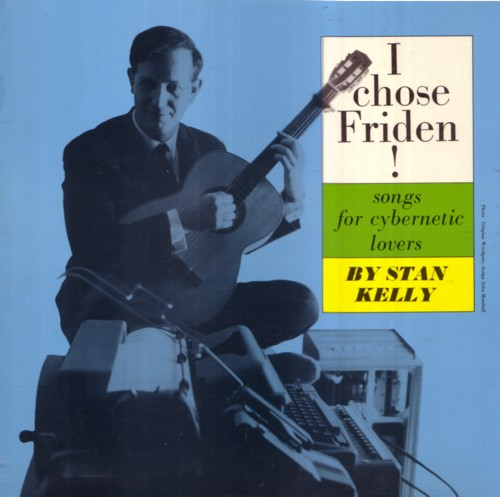
\includegraphics[width=4cm]{fig/kelly.jpg}
      
      \textit{``Should array indices start at 0 or 1 ? 
My compromise of 0.5 was rejected without, I thought, proper consideration''}\\
      \small{
        \hfill Stan Kelly-Bootle (1929-2014)\\
               \hfill informaticien, auteur-compositeur}
    }
  \end{columns}
  
\end{frame}

\begin{frame}
\frametitle{G�n�ralit�s}
\begin{itemize}
  \setlength\itemsep{1em}
\item Un tableau est un ensemble d'�l�ments de m�me type
d�sign� par un identificateur unique.\\
\item Chaque �l�ment est rep�r� par un \red{indice} pr�cisant
sa position au sein de l'ensemble.\\
\item Il se d�clare en m�me temps que les autres variables.\\
\item Il existe deux grandes familles de tableaux : \\
\begin{itemize}
\item Les tableaux unidimensionnels (vecteurs)\\
\item Les tableaux multidimensionnels (matrices)\\
\end{itemize}
\end{itemize}
\end{frame}

\begin{frame}[fragile]
\frametitle{D�claration de tableaux unidimensionnels}
\begin{itemize}
\item On doit r�server un emplacement m�moire pour un certain
nombre d'�l�ments.\\
{\centering{
\bvrb|�textit�type nom_tableau�[ �textit�nb_elements� ];|\\
}}
\begin{itemize}
\item \bvrb|�textit�type�| est le type des �lements du tableau \bvrb|�textit�nom_tableau�|\\
\item \bvrb|�textit�nb_elements�| est le nombre d'�l�ments que contient le tableau.\\
\end{itemize}

\item Conventionnellement, \red{la premi�re position porte le num�ro 0}.
Les indices vont donc de \verb|0| � \Verb|nb_elements-1|
\end{itemize}
\begin{codeblock}{}
%\vspace{-.3cm}
\lstset{escapeinside={��}}
%\lstset{basicstyle=\scriptsize}
\begin{codeC}
int tab[10] ; // tab est un tableau de 10 entiers
float zz[5] ; // zz est un tableau de 5 r�els
char y[12] ; // y est un tableau de 12 caract�res
\end{codeC}
\end{codeblock}
\end{frame}

\begin{frame}
\frametitle{Quelques r�gles}
\begin{itemize}
 \setlength\itemsep{1em}
\item Chaque �l�ment est stock� dans une case d'un tableau
(localis� par un \red{indice}).\\
\item Un �l�ment de tableau est une variable :
\begin{itemize}
\item On peut l'initialiser.\\
\item On peut l'utiliser dans une expresssion.\\
\end{itemize}
\item Le premier �l�ment du tableau est � l'indice \red{0}.\\
\item La dimension d'un tableau (nombre d'�l�ments) ne peut �tre
qu'une constante ou une expression constante (pas une variable).\\
\item Il faut faire tr�s attention aux probl�mes de d�bordement d'indice
(cas o� l'on veut acc�der � un indice de tableau sup�rieur au nombre
d'�l�ments pr�vus).\\
\end{itemize}

\end{frame}

\begin{frame}[fragile]
\frametitle{Initialisation des �l�ments (1)}

\begin{itemize}
\item Initialisation de l'�lement d'indice \verb|k| :\\

\begin{columns}
\column{0.5\textwidth}
\begin{block}{}
\bvrb|�textit�nom_tableau�[k] = �textit�valeur� ;|\\
\bvrb|�textit�nom_tableau�[k] = �textit�expression� ;|\\
\end{block}
\column{0.45\textwidth}
\begin{codeblock}{}
\vspace{-.3cm}
\lstset{escapeinside={��}}
\lstset{basicstyle=\scriptsize}
\begin{codeC}
tab[0]=5 ;
/* le premier �l�ment du 
tableau tab a pour 
valeur 5*/
\end{codeC}
\vspace{-.3cm}
\end{codeblock}
\end{columns}
\item Initialisation � la d�claration
\begin{codeblock}{}
\vspace{-.3cm}
\lstset{escapeinside={��}}
\lstset{basicstyle=\scriptsize}
\begin{codeC}
//Place les valeurs 1,2,3,4,5 dans chacun des 
//5 �l�ments du tableau :
int tab[5] = {1,2,3,4,5};

//Ne remplit que certains indices (ici 2 et 4) :
int tab[5] = {,,3,,5};

//Ne remplit que les 2 premiers indices (0 et 1) :
int tab[5] = {2,3};

//Determine automatiquement la taille du tableau (en fonction
//du nombre de valeurs :
int tab[] = {1,2,3,4,5};

\end{codeC}
\vspace{-.3cm}
\end{codeblock}
\end{itemize}

\end{frame}

\begin{frame}[fragile]
\frametitle{Initialisation des �l�ments (2)}
\begin{block}{}
Initialisation des �l�ments dans une boucle \bvrb|for|
\end{block}
\begin{columns}[t]
\column{0.45\textwidth}
\begin{table}
\centering
\begin{tabular}{|c|c|c|c|c|}
\hline
0 & 0 & 0 & 0 & 0 \\
\hline
\end{tabular}
\end{table}
\begin{codeblock}{}
\vspace{-.3cm}
\lstset{escapeinside={��}}
%\lstset{basicstyle=\scriptsize}
\begin{codeC}
int j ; //ind. de boucle
int Tab[5] ;

for (j=... ; ... ; ...) 

{

...

}

\end{codeC}
\vspace{-.3cm}
\end{codeblock}

\column{0.45\textwidth}
\begin{table}
\centering
\begin{tabular}{|c|c|c|c|c|}
\hline
0 & 2 & 4 & 6 & 8 \\
\hline
\end{tabular}
\end{table}
\begin{codeblock}{}
\vspace{-.3cm}
\lstset{escapeinside={��}}
%\lstset{basicstyle=\scriptsize}
\begin{codeC}
int j ; //ind. de boucle
int Tab[5] ;

for (j=... ; ... ; ...) 

{

...

}

\end{codeC}
\vspace{-.3cm}
\end{codeblock}

\end{columns}

\end{frame}

\begin{frame}[fragile]
\frametitle{Un exemple (version 1)}
\begin{columns}
\column{0.5\textwidth}
\begin{codeblock}{}
\vspace{-.3cm}
\lstset{escapeinside={��}}
\lstset{basicstyle=\scriptsize}
\begin{codeC}
#include <stdio.h>

/* Remplissage d'un tableau de
notes et calcul de la moyenne */

int main()
{
  float notes[50], moy=0.0;
  int i;
  
  for (i=0;i<50;i++)
  {
    printf("\Entrez la note: ");
    scanf("%f",&notes[i]);
    moy += notes[i];
  }
  printf("\nmoyenne = %f",moy/50);
}
\end{codeC}
\vspace{-.3cm}
\end{codeblock}

\column{0.5\textwidth}
\begin{itemize}
\item On remplit les 50 �l�ments du 
tableau (utilisation d'une boucle
\bvrb|for|)\\
\item \Verb|i| sert d'indice pour parcourir
les �l�ments du tableau.\\
\item La moyenne est calcul�e en ajoutant
� chaque pasasge de boucle, la nouvelle 
note saisie au clavier (\bvrb|scanf|)\\
\end{itemize}

\end{columns}

\end{frame}

\begin{frame}[fragile]
\frametitle{Probl�mes dans l'exemple}
\begin{itemize}
 \setlength\itemsep{1em}
\item Utilisation non s�curis�e de \bvrb|scanf|\\
\begin{itemize}
\item V�rification du nombre d'�l�ments correctements
entr�s
\item "Nettoyage de la m�moire tampon".\\
\end{itemize}
\item Probl�me pratique si on veut modifier la taille
du tableau.\\
\end{itemize}
\end{frame}


\begin{frame}[fragile]
\frametitle{Un exemple (version 2)}
\begin{columns}
\column{0.5\textwidth}
\begin{codeblock}{}
\vspace{-.3cm}
\lstset{escapeinside={��}}
\lstset{basicstyle=\scriptsize}
\begin{codeC}
#include <stdio.h>
#define NMAX 50

/* Remplissage d'un tableau de
notes et calcul de la moyenne */

int main()
{
  float notes[NMAX], moy=0.0;
  int i;
  
  for (i=0;i<NMAX;i++)
  {
    printf("\Entrez la note: ");
    scanf("%f",&notes[i]);
    moy += notes[i];
  }
  printf("\nmoyenne = %f",moy/NMAX);
}
\end{codeC}
\vspace{-.3cm}
\end{codeblock}

\column{0.45\textwidth}
D�finition de la taille du 
tableau par un \bvrb|#define| (fortement
conseill�).\\

\begin{alertblock}{}
Si la valeur de \Verb|NMAX| est modifi�e,
il faut recompiler.
\end{alertblock}
\end{columns}

\end{frame}

\begin{frame}[fragile]
\frametitle{Les tableaux multidimensionnels}
\begin{block}{D�claration}
\bvrb|�textit�type nom_tableau �[�textit�dim1�][�textit�dim2�]...[�textit�dimN�];|
\end{block}

\begin{codeblock}{Initialisation}
\vspace{-.3cm}
\lstset{escapeinside={��}}
\lstset{basicstyle=\scriptsize}
\begin{codeC}
//tableau vu comme 5 tableaux de deux �l�ments chacun
int tab[5][2] = {{1,2},{3,4},{5,6},{7,8},{9,10}};

//El�ments rang�s en m�moire automatiquement :
int tab[5][2] = {1,2,3,4,5,6,7,8,9,10};

//Omission de valeurs :
int tab[5][2] = {1,,3,,,,7,8,9,};

//Acc�s � un indice (apr�s d�claration):
tab[3][0] = 12 ;

\end{codeC}
\vspace{-.3cm}
\end{codeblock}

\end{frame}

\begin{frame}
\frametitle{Algorithmes classiques sur les tableaux}
\begin{itemize}
 \setlength\itemsep{1em}
\item Initialisation d'un tableau � une valeur constante.\\
\item Copie d'un tableau.\\
\item V�rification de l'�galit� de deux tableaux.\\
\item Recherche d'un �l�ment dans un tableau.\\
\item Comptage du nombre d'occurences d'un �l�ments
dans un tableau.\\
\item Tri des �l�ments dans un tableau.\\
\end{itemize}
\end{frame}
\end{document} 

%%%%%%%%%%%%%%%%%%%%% SECTION 1
\section{Les algorithmes}\label{section:1}
\begin{frame}
\begin{columns}
        \column{4.8cm}
            \tableofcontents[currentsection]
        \column{7cm}
        \centering{
            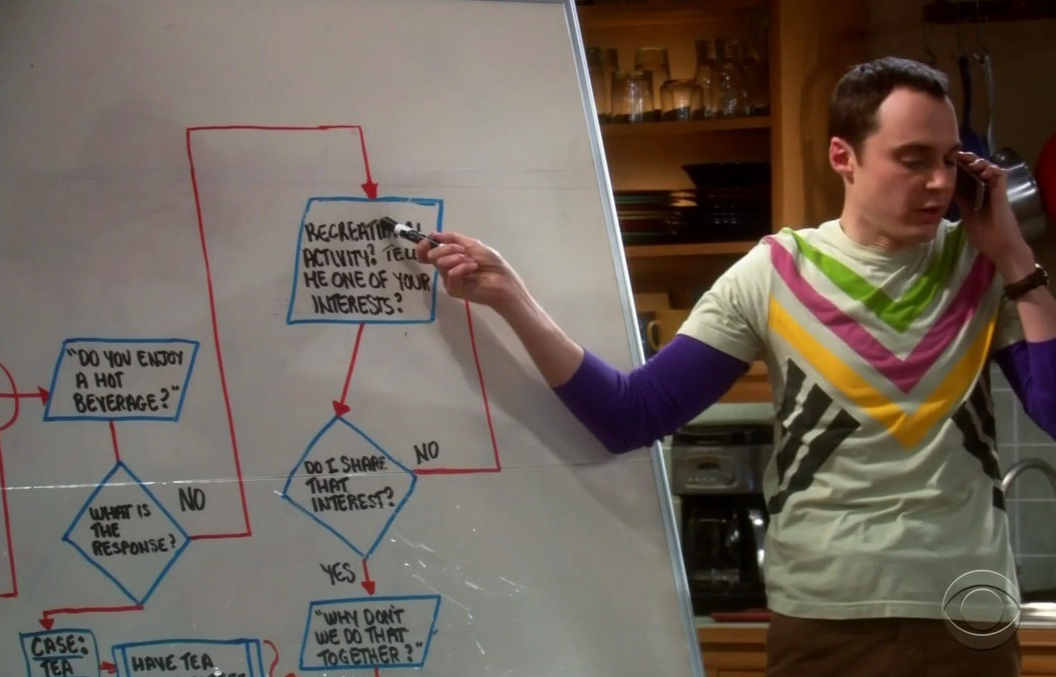
\includegraphics[width=7cm]{fig/Algorithm-sheldon.png}
            
                 \textit{ I believe I've isolateblblblblblblsblbslbslbsl
            sblbslblsblsblblsblbs
            lbslblbslsb d the algorithm for making friends.}
     
            
            \small{
            \hfill Sheldon Cooper, 
            
            \hfill in \textit{The Big Band Theory}, Season 2, Episode 13
            }
}

    \end{columns}

\end{frame}


%%%%%%%%%%%%%%%%%%%%%
\subsection{Introduction}
    \begin{frame}
    \frametitle{Pourquoi faire appel � des algorithmes ?}
    Pour automatiser des t�ches
    
    Exemples :
    \begin{itemize}
    \item M�tier � tisser\\
    \item M�thode de calcul � la main d'une division\\
    \item Recette de cuisine\\
    \item ...\\
    \end{itemize}
    \end{frame}
 
 %%%%%%%%%%%%%%%%%
 
    \begin{frame}
    \frametitle{Qu'est-ce qu'un algorithme ?}
    \begin{block}{D�finition}
    Un algorithme est un ensemble 
    ordonn� d'instructions simples
permettant de r�soudre un probl�me.
    \end{block}
    \end{frame}
    
 %%%%%%%%%%%%%%%%%%
 \subsection{Construction d'un algorithme}
%%%%%%%%%%%%%%%%%%%    
\section{La machine de Turing}
%%%%%%%%%%%%%%%%%%%%
 
  
\begin{frame}[fragile]
\frametitle{Un peu d'histoire...}
\begin{codeblock}{Test}
\begin{codeC}
for (int i = 0 ; i < n ; i ++) {
    //a comment
    printf("%d",i);
    }
\end{codeC}
\end{codeblock}

\begin{termblock}{test 2}
\lstset{escapeinside={��}}
\begin{lstlisting}
�\textbf{>>}�./a.out
�\color{darkgray}{\texttt{  Hello World}}�
\end{lstlisting}
\end{termblock}

 \begin{block}{Bloc standard}
blablabla
\end{block}
\end{frame}


\begin{frame}[fragile]
\frametitle{essai}
\begin{columns}
\column{6cm}
\begin{block}

\begin{figure}
\begin{tikzpicture} [
    auto,
    decision/.style = { diamond, draw=blue, thick, fill=blue!20,
                        text width=5em, text badly centered,
                        inner sep=1pt, rounded corners },
    block/.style    = { rectangle, draw=blue, thick, 
                        fill=blue!20, text width=10em, text centered,
                        rounded corners, minimum height=2em },
    line/.style     = { draw, thick, ->, shorten >=2pt },
  ]
   \matrix [column sep=-10mm, row sep=10mm] {
                    & \node [text centered] (x) {$\mathbf{X}$};            & \\
                    & \node (null1) {};                                    & \\
                    & \node [block] (doa) {\textsf{DoAE}($\mathbf{X}$)};   & \\
  	               \node(null3){}; & \node [decision] (uiddes)
                        {\textsf{UID}($\hat{\mathbf{X}}$)};
                                  & \node[text centered](tra){$\mathbf{i}$}; \\
                  & \node [block] (track) {\textsf{DoAT}($\mathbf{x}$)}; & \\
                    & \node [block] (pesos)
                        {\textsf{BF}(DoA$_{\mathrm{T}}$,DoAs)};            & \\
                    & \node [block] (filtrado)
                        {\textsf{SF}($\mathbf{w}$,$\mathbf{x}$)};          & \\
                    & \node [text centered] (xf) {$\hat{x}(t)$ };          & \\
  };
  % connect all nodes defined above
 \begin{scope} [every path/.style=line]
    \path (x)        --    (doa);
    \path (doa)      --    node [near start] {DoAs} (uiddes);
    \path (tra)      --    (uiddes);
    \path (uiddes)   --++  (-3,0) node [near start] {no} |- (null1);
    \path (uiddes)   --    node [near start] {DoA} (track);
    \path (track)    --    node [near start] {DoA$_{\mathrm{T}}$} (pesos);
    \path (pesos)    --    node [near start] {\textbf{w}} (filtrado);
    \path (filtrado) --    (xf);
  
  \end{scope}
\end{tikzpicture}
\end{figure}
\end{block}
\column{3cm}
\begin{block}{bulbul}
\end{block}
\end{columns}
\end{frame}

\end{document}
